\documentclass[tikz,border=5]{standalone}
\usepackage{eulervm}
\usepackage[osf,sc]{mathpazo}
\usepackage{inconsolata}
\usetikzlibrary{matrix}
\begin{document}
	\tikzset{
		entity/.code={
			\tikzset{
				rounded corners,             
				name=#1,
				inner sep=2pt,
				every entity/.try,
			}%
			\def\entityname{#1}%
		},
		elabel/.style = {
			above,midway,sloped
		},
		eprop/.style = {
			draw=black, text width=2.2cm, below, midway, sloped
		},
		entity anchor/.style={matrix anchor=#1},
		every entity/.style={
			draw,
		},
		every property/.style={
			inner xsep=0.20cm, inner ysep=0.075cm, anchor=west, text width=1.75in
		}
	}
	\def\property#1{\node[name=\entityname-#1, every property/.try]{\propertysplit#1;};}
	\def\properties{\begingroup\catcode`\_=11\relax\processproperties}
	\def\processproperties#1{\endgroup%
		\gdef\propertycode{}%
		\foreach \p in {#1}{%
			\expandafter\expandafter\expandafter\gdef\expandafter\expandafter\expandafter\propertycode%
			\expandafter\expandafter\expandafter{\expandafter\propertycode\expandafter\property\expandafter{\p}\\}%
		}%
		\propertycode%
	}
	\def\propertysplit#1:#2;{\textbf{#1}:#2}
	
	\def\entitynamenode{%
		\node[every entity name/.try] (\entityname-name) {\textbf{\entityname}};
		\draw (\entityname-name.south west) -- (\entityname-name.south east);
		\\[1ex]
	}
	\tikzset{
		every entity name/.style={every property/.try, align=center}
	}
	
	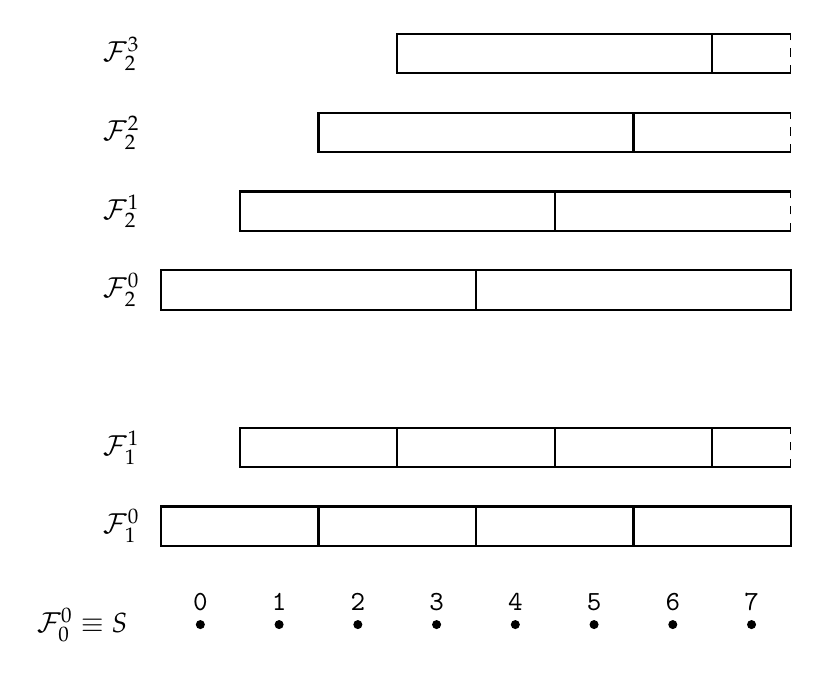
\begin{tikzpicture}[every node/.style={font=\ttfamily}, node distance=1cm]
	
	\node[] at (-1.5,0) {$\mathcal{F}^0_0\equiv S$};
\node[inner sep=1pt,circle,draw,fill,label={0}] (a0) {};
\node[inner sep=1pt,circle,draw,fill,label={1},right of=a0] (a1) {};
\node[inner sep=1pt,circle,draw,fill,label={2},right of=a1] (a2) {};
\node[inner sep=1pt,circle,draw,fill,label={3},right of=a2] (a3) {};
\node[inner sep=1pt,circle,draw,fill,label={4},right of=a3] (a4) {};
\node[inner sep=1pt,circle,draw,fill,label={5},right of=a4] (a5) {};
\node[inner sep=1pt,circle,draw,fill,label={6},right of=a5] (a6) {};
\node[inner sep=1pt,circle,draw,fill,label={7},right of=a6] (a7) {};

	\node[] at (-1,1.25) {$\mathcal{F}^0_1$};
	\draw[thick] (-0.5,1) rectangle (1.5,1.5);
	\draw[thick] (1.5,1) rectangle (3.5,1.5);
	\draw[thick] (3.5,1) rectangle (5.5,1.5);
	\draw[thick] (5.5,1) rectangle (7.5,1.5);
	\node[] at (-1,2.25) {$\mathcal{F}^1_1$};
	\draw[thick] (0.5,2) rectangle (2.5,2.5);
	\draw[thick] (2.5,2) rectangle (4.5,2.5);
	\draw[thick] (4.5,2) rectangle (6.5,2.5);
	\draw[thick] (7.5,2) -- (6.5,2) -- (6.5,2.5) -- (7.5,2.5);
	\draw[dashed] (7.5,2) --  (7.5,2.5);

\node[] at (-1,4.25) {$\mathcal{F}^0_2$};
\draw[thick] (-0.5,4) rectangle (3.5,4.5);
\draw[thick] (3.5,4) rectangle (7.5,4.5);
\node[] at (-1,5.25) {$\mathcal{F}^1_2$};
\draw[thick] (0.5,5) rectangle (4.5,5.5);
\draw[thick] (7.5,5) -- (4.5,5) -- (4.5,5.5) -- (7.5,5.5);
\draw[dashed] (7.5,5) --  (7.5,5.5);
\node[] at (-1,6.25) {$\mathcal{F}^2_2$};
\draw[thick] (1.5,6) rectangle (5.5,6.5);
\draw[thick] (7.5,6) -- (5.5,6) -- (5.5,6.5) -- (7.5,6.5);
\draw[dashed] (7.5,6) --  (7.5,6.5);
\node[] at (-1,7.25) {$\mathcal{F}^3_2$};
\draw[thick] (2.5,7) rectangle (6.5,7.5);
\draw[thick] (7.5,7) -- (6.5,7) -- (6.5,7.5) -- (7.5,7.5);
\draw[dashed] (7.5,7) --  (7.5,7.5);

	\end{tikzpicture}   
	
\end{document}
